
\documentclass[preprint,11pt]{elsarticle}


\usepackage{fullpage} % Package to use full page
\usepackage{parskip} % Package to tweak paragraph skipping
\usepackage{tikz} % Package for drawing
\usepackage{amsmath}
\usepackage{hyperref}
\usepackage{xcolor}
\usepackage{listings}


\journal{PEC1}
\begin{document}
\begin{frontmatter}

    \title{Pec1: Temas M1-M2-M3}
    \author{Marc brunet presas}
    \address{Manresa, Barcelona,}
    \begin{abstract}
    Esta primera PEC consiste en una aproximación al mundo GNU/Linux, siguiendo los contenidos marcados en el primer módulo de la asignatura. En ella, deberemos reflexionar sobre los diferentes tipos de distribución y hacer una serie de instalaciones.
    \end{abstract}
\end{frontmatter}


%% main text
\section{Ejercicio 1}
\label{S:1}
Para esta pregunta es necesario documentarse sobre la distribución Debian, Fedora y Suse.
\subsection{Realizar una comparativa entre las licencias de usuario final (EULA) de estas distribuciones que pueden presentar por ejemplo en forma de tabla. Qué conclusiones pueden obtener de esta comparación y cuale son las posibles consecuencias?}

\begin{tabular}{ |p{5cm}||p{2cm}|p{2cm}|p{2cm}|  }
 \hline
 \multicolumn{4}{|c|}{distributions} \\
 \hline
  &Debian &Fedora &Suse\\
 \hline
Components no lliures &si &si &-\\
pagaments de codi font &no &si &-\\
pagaments de descarrega &no &no &si\\
suport &comunitat &comunitat &si \\
 \hline
\end{tabular}
\bigskip 

al analizar un poco las licencias de canda uno de los sistema vemos que algunos son mantenidos i gestionados totalmente por una comunidad como Debian o Fedora i Suse con una empresa como deparas sacando beneficio dando soporte como en una empresa tradicional, vendiendo sus productos i manteniendolos 


\newpage
\subsection{b. Analizar las páginas web de las tres distribuciones. Definir en forma precisa cual es el objetivo de cada distribución y que servicios se están ofreciendo a sus usuarios}
\label{S:2}

\paragraph{Debian}\footnote{https://www.debian.org/} sistema operativo conocido pero la poca facilidad i las ultimas novedades, pagina web muy identificativa de esta mentalidad muy esquemática con toda la información en la pagina principal, también los enlaces a las descargas de las ultimas versiones del sistema, una pagina muy encarada a la funcionalidad i a los usuarios mas experimentados para buscar las ultimas noticies versiones o comentarios 

\paragraph{Fedora}\footnote{https://getfedora.org/}pagina con estética moderna i con información de las versiones disponibles, separan en 3 versiones para Workstation o personal, server para el uso con servidores o centros de datos, i atom versión muy minimalista para montar servicios basodos en contenedores, también muestran imágenes ARM, para usar en dispositivos enveded para IOT o micro ordenadores, muestran una imagen de un producto muy completo i disponible para todas las plataformas o caso de uso.\bigskip

Workstation: versión diseñada para el uso diario profesional o personal, con eramientas para facilitar el trabado i entornos visuales agradables i fáciles de usar con tecnologías de virtualización i docker\bigskip

server: ofrecen diversas versiones con diversos ciclos de vida para adaptarse despacio o rápidamente a los cambios, usado Modularity para gestionar los ciclos de vida independientemente por paquete, i eramientas de administración i bases de datos\bigskip

atom: es una versión muy reducida diseñada expresamente para  LDK (Linux-Docker-Kubernetes)\bigskip

\paragraph{Suse}\footnote{https://www.suse.com} página de estilo corporativa da la sensación de vender un producto con una empresa detrás, ofrece servicios de atención al cliente desde la primera página, con información de usos de usos de sus productos un blog informativo y caso de éxito de sus productos. Dispone de un catalogo de productos ordenado pero necesidades para poder ofrecer el producto más interesante, vende sus productos por versiones Y son extensibles por paquetes, dispone de versiones para el Workstation o personal asta la implementación en la nube, pasado por almacenamiento o gestión de las infraestructuras en la empresa. Están muy encarados a sistemas para empresas. \bigskip

\subsection{c. A partir de esta información proponga tres situaciones de instalación en las cuales aconsejaría utilizar una de estas distribuciones justificando de forma razonada esta propuesta}\bigskip

depures de analizar un poco cada una de les distribuciones recomendaría suse para una empresa que está en planeando una migración de Windows O mac os x , ja que dispone de características muy parecidas, como un puesto de respuesta y resolución de problema, seguramente tendra un sistema de orientación y acompañamiento en la migración, aparte dispone productos para todas las necesidades en una sola compañía, seria un soporte y migración, seria una migración completa en todos los aspectos desde los departamentos más tecnológicos asta los más administrativos, ofreciendo respuesta a los departamentos de IT en la gestión y mantenimiento de la maquinas, a los desabolladores en el sistema operativo y en los administradores en el aspecto gráfico y sus herramientas de ofimáticas.\bigskip

fedora lo recomendaría en una empresa tecnológica que este planeado un migración ofrece sistemas Workstation y servers con la posibilidad de ir a los microservision, tendrían que ser una empresa con mentalidad moderna y con un objetivo de modernización en sus planes de futuro, tendran que estar modernizado el software constantemente sin un soporte oficial i deberán apoyarse de la comunidad, teniendo opciones de dejar parte del sistema en una versión antigua. La parte más tecnológica de la empresa no tendrá problemas pero la parte más administrativa puede tener algún problema de compatibilidad i tendrá que solucionarlo la parte más tecnología pero tanto puede plantearse una migración parcial\bigskip


debian solo lo recomendaría en usuaria avanzados todo i que te una parte estable puede ser bastate complicado una actualización o inhalación, seria una migración domes de la Prat mes tecnología de la empresa incluso solo los servidores en algún caso o también los miembros de IT i desabolladores\bigskip

\subsection{ Comentar para cada una de ella y de la información previa el rango de uso de cada distribución (se puede seguir el formato tal y como aparece en la página de Distrowatch http://distrowatch.com pero debe ser elaborado con la información previa que han analizado.}\bigskip


\begin{tabular}{ |p{4cm}||p{3cm}|p{3cm}|p{3cm}|  }
 \hline
 \multicolumn{4}{|c|}{distributions} \\
 \hline
  &Workstation  &Server  &Cloud \\
 \hline
Debian &si &si &si\\
Fedora Workstation  &si &no &no\\
Fedora Server &no &si &si\\
Fedora atom &no &si &si \\
suse &si &si &si \\
 \hline
\end{tabular}
\bigskip 

fedora con las versiones atom i server pueden usarse en servidores locales para obtener un servidor local con aplicaciones tradicionales, o contenedores, indistintamente, todo i que cada versión esta más encara da cada uso particular.\bigskip

devian como tal puede usarse indistintamente en cualquier parte pero la complicación de no disponer de una versión especifica puede complicar las tareas de configuración i instalación de los entornos.\bigskip

suse puede usarse en todos los entornos dispone versiones especificas para cada uso y extensibles con paquetes extras, lo que lo hace perfectamente adaptable a cada uso.\bigskip

\clearpage
\section{Ejercicio 2}
Para esta parte práctica, se deberá hacer al menos dos instalaciones de GNU/Linux, en una configuración de escritorio (no pensado para servidor) y con un mismo gestor de ventanas en los dos casos (Gnome, KDE, o el que deseen – pero que sea el mismo en todas las instalaciones). Se deberán de entre las siguientes tres posibles ramas: Fedora/CentOS, Debian/Ubuntu o Suse. Para algunas distribuciones pueden usar el material distribuido con la asignatura, descargar otras imágenes directamente desde Internet oaprovechar material que ya tengan disponible. En todo caso, habra que usar imágenes de CD/DVD de instalación, y no una imagen completa de sistema ya preparada por su ejecución.\bigskip

\subsection{a. Documentar el proceso de instalación: qué diferencias mayores han encontrado en el software para hacer la instalación, qué problemas han detectado (dispositivos que no funcionan, resolución, etc) y qué soluciones han buscado y aplicado. Como muestra del funcionamiento de deberá mostrar en un terminal la ejecución de comando uname -a y se debe mostrar que pueden navegar a una página de Internet actualizada (donde se indique claramente la fecha y hora, por ejemplo a un diario) }

Realizado y documentado en el anexo, Todo y que en la inhalación de los sistemas ubuntu 18.04 y fedora workstation 29 no he tendió problemas con ningún adaptador ni dispositivo cuando he instalado ubuntu en algún portátil he tenido problemas con las tarjetas gráfica nvidia y algunos adaptadores de wifi nada que con descargase los controladores adicionales públicos o privativos no pudiera solucionar

\subsection{b. Examinar el sistema de ficheros y realizar una tabla comparativa de: qué diferencias han detectado entre las dos instalaciones? Qué ocupación del disco tienen – y, si hay variaciones, como las pueden explicar?}
ejecutamos:


\clearpage
\section{bibliografía}
    \textbf{URLS:}
    \begin{itemize}
        \item web del proyecto suse https://www.suse.com consulta 30/oct/2018
        \item web del proyecto getfedora https://www.getfedora.org consulta 30/oct/2018
        \item web del proyecto debian  https://www.debian.org consulta 30/oct/2018
        \item Web de consulta de distribuciones https://distrowatch.com consulta 30/oct/2018
    \end{itemize}

\clearpage
\section{Anex}
\subsection{Ubuntu 18.04}
\begin{figure}[!htbp]
    \begin{center}
        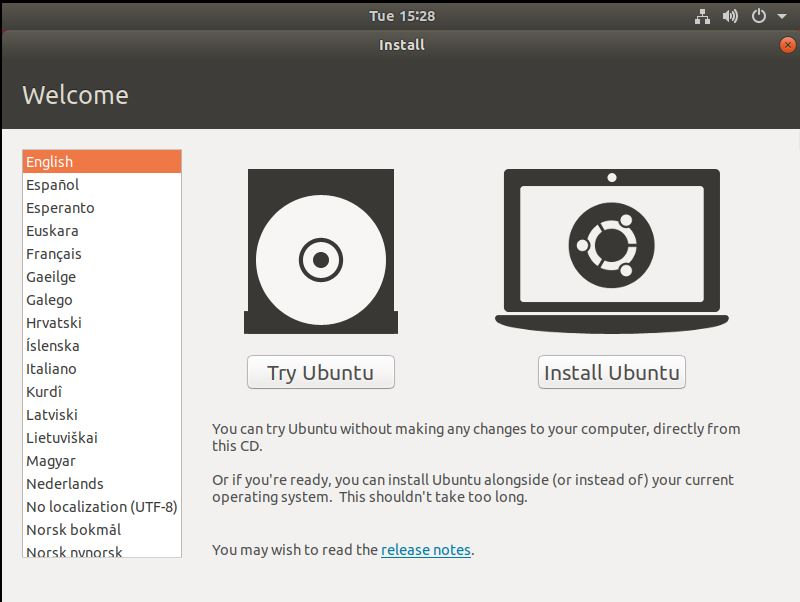
\includegraphics[width=11cm]{anex/ubuntu1.JPG}
    \end{center}
    \caption{Escogemos si lo probamos o lo instalamos y la distribución del teclado}
    \begin{center}
        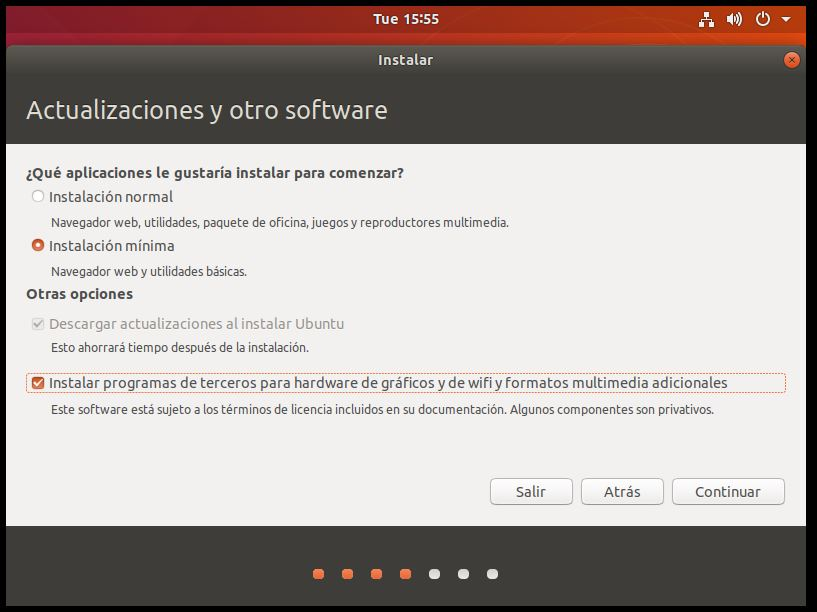
\includegraphics[width=11cm]{anex/ubuntu2.JPG}
    \end{center}
    \caption{Una vez seleccionado el idioma escomeremos la distribución del teclado y procedemos al tipo de instalación que queremos, y si deseamos incluir programas de 3r (que pueden contener licencias privativas)}
\end{figure}
\begin{figure}[!htbp]
    \begin{center}
        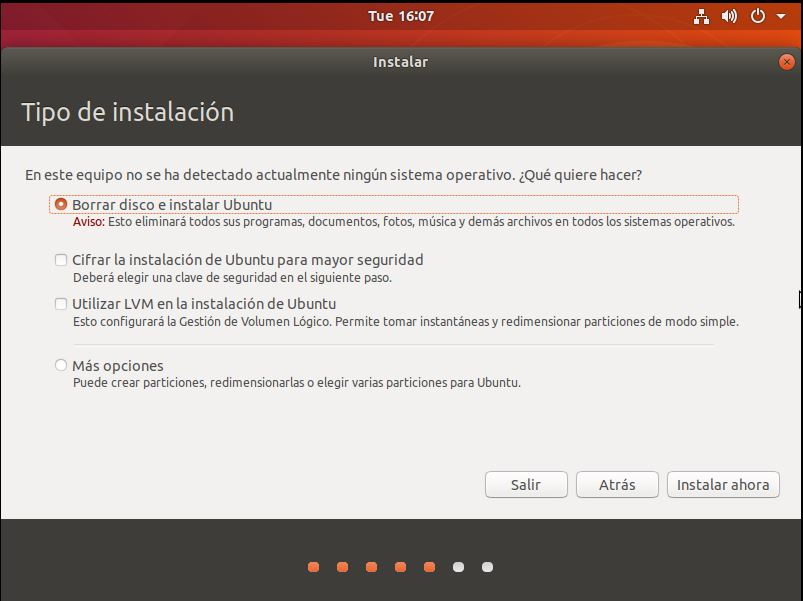
\includegraphics[width=11cm]{anex/ubuntu3.JPG}
    \end{center}
    \caption{Nos permite selección un formateo del disco automático o escoger el formato que no nosotros queremos}
    \begin{center}
        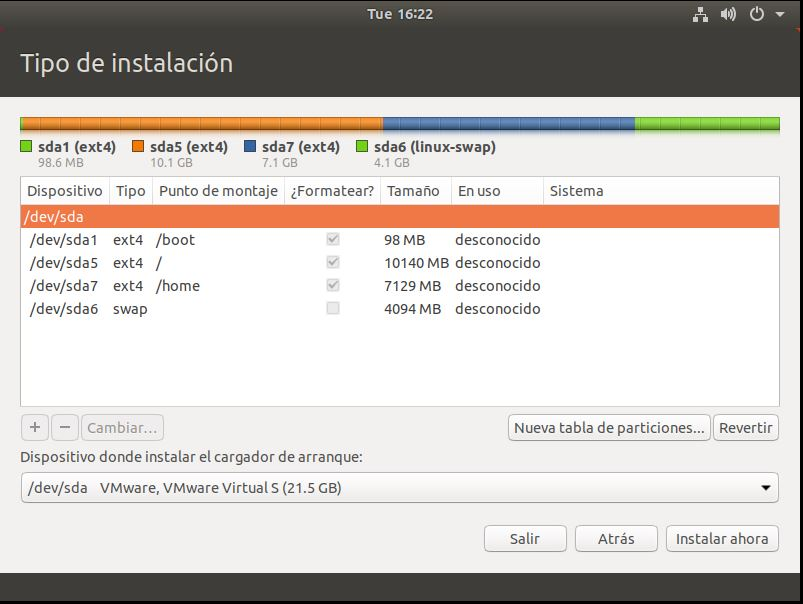
\includegraphics[width=11cm]{anex/ubuntu4.JPG}
    \end{center}
    \caption{Podemos configurar las particiones en el formato que queramos una partición para todo el sistema o frentes particiones para las carpetas generales}
\end{figure}

Haremos unas configuraciones básicas de nombre de usuario y credenciales nombre de maquina y ubicación, y el poseso de instalación seguirá y actualizará la maquina asta que no pida el reinicio

\begin{figure}[!htbp]
    \begin{center}
        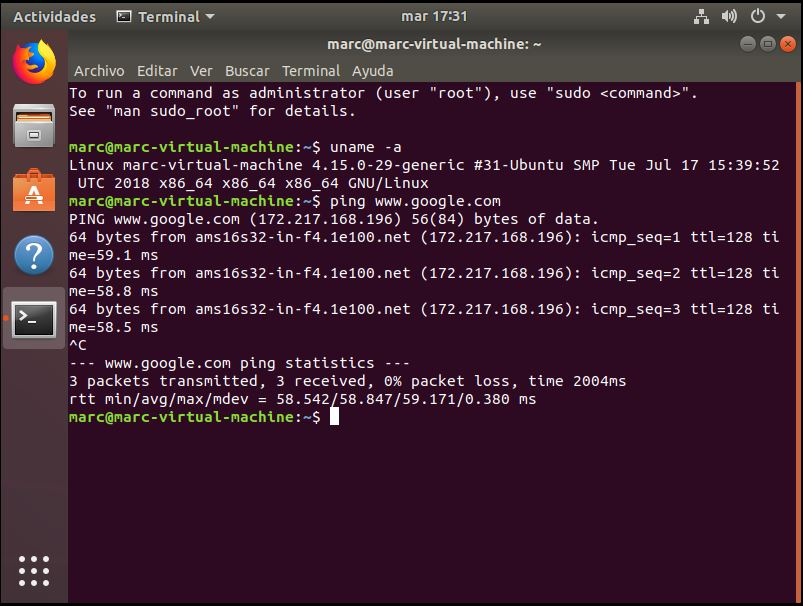
\includegraphics[width=11cm]{anex/ubuntu5.JPG}
    \end{center}
    \caption{,ejecución del comando uname -a y un ping a google.com}
    \begin{center}
        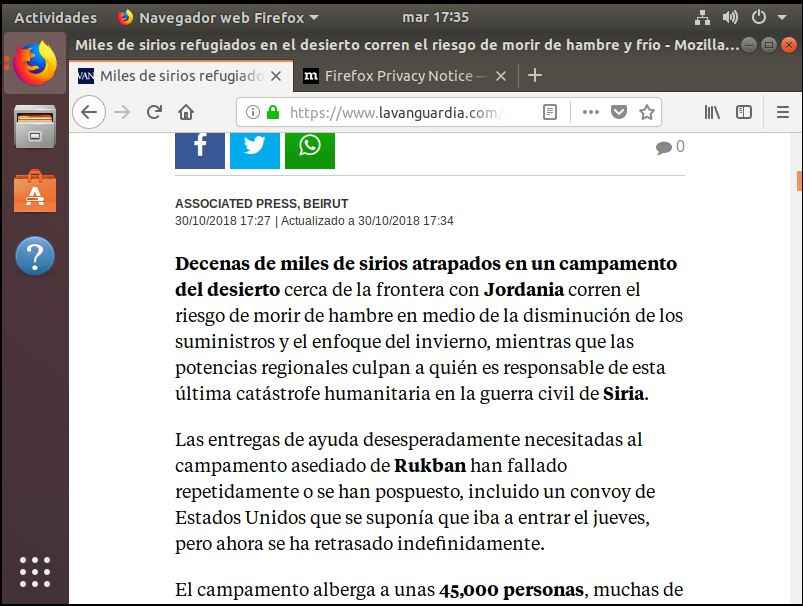
\includegraphics[width=11cm]{anex/ubuntu6.JPG}
    \end{center}
    \caption{comprobación de una noticia de la vanguardia \newline https://www.lavanguardia.com/internacional/20181030/452657349845/siria-campamento-rukban-hambre-frio.html}
\end{figure}

\clearpage
\subsection{Fedora 29}
\begin{figure}[!htbp]
    \begin{center}
        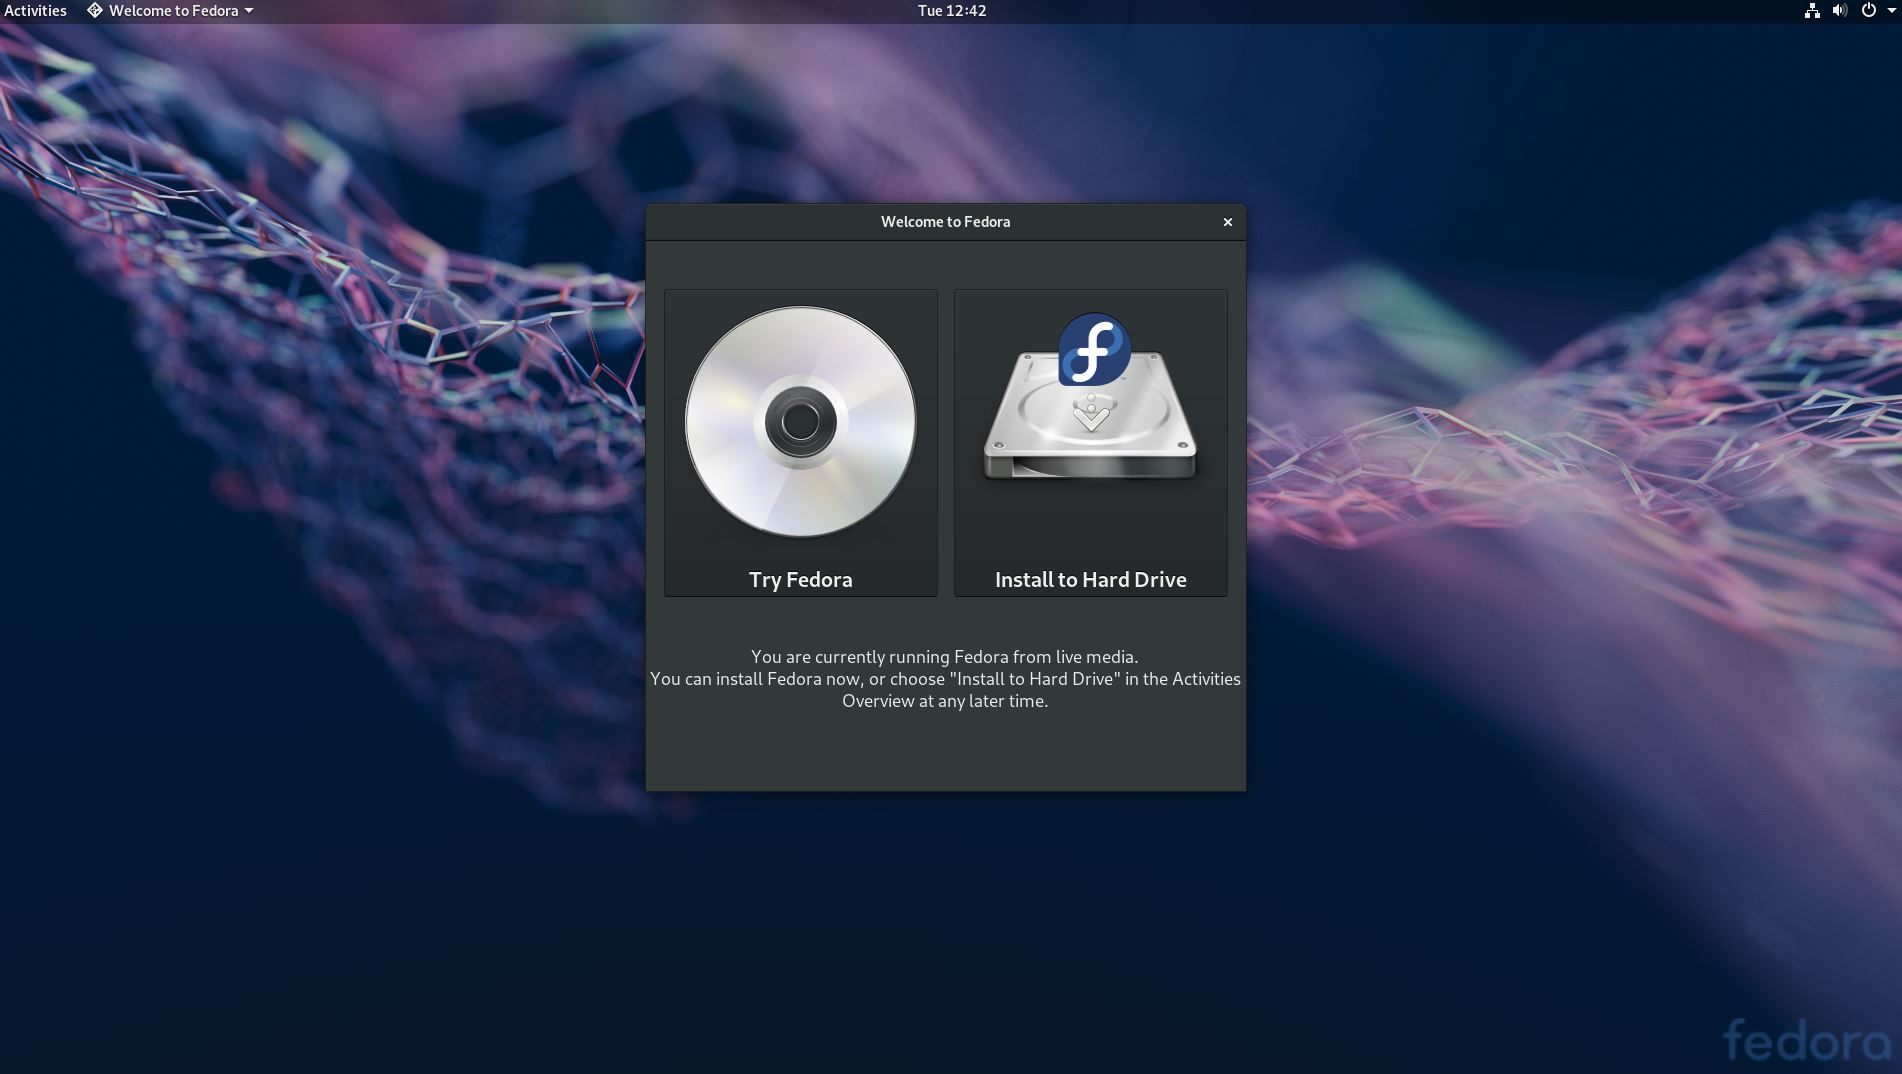
\includegraphics[width=11cm]{anex/fedora1.JPG}
    \end{center}
    \caption{Pantalla inicial de la inhalación de fedroa podemos instalar o probar }
    \begin{center}
        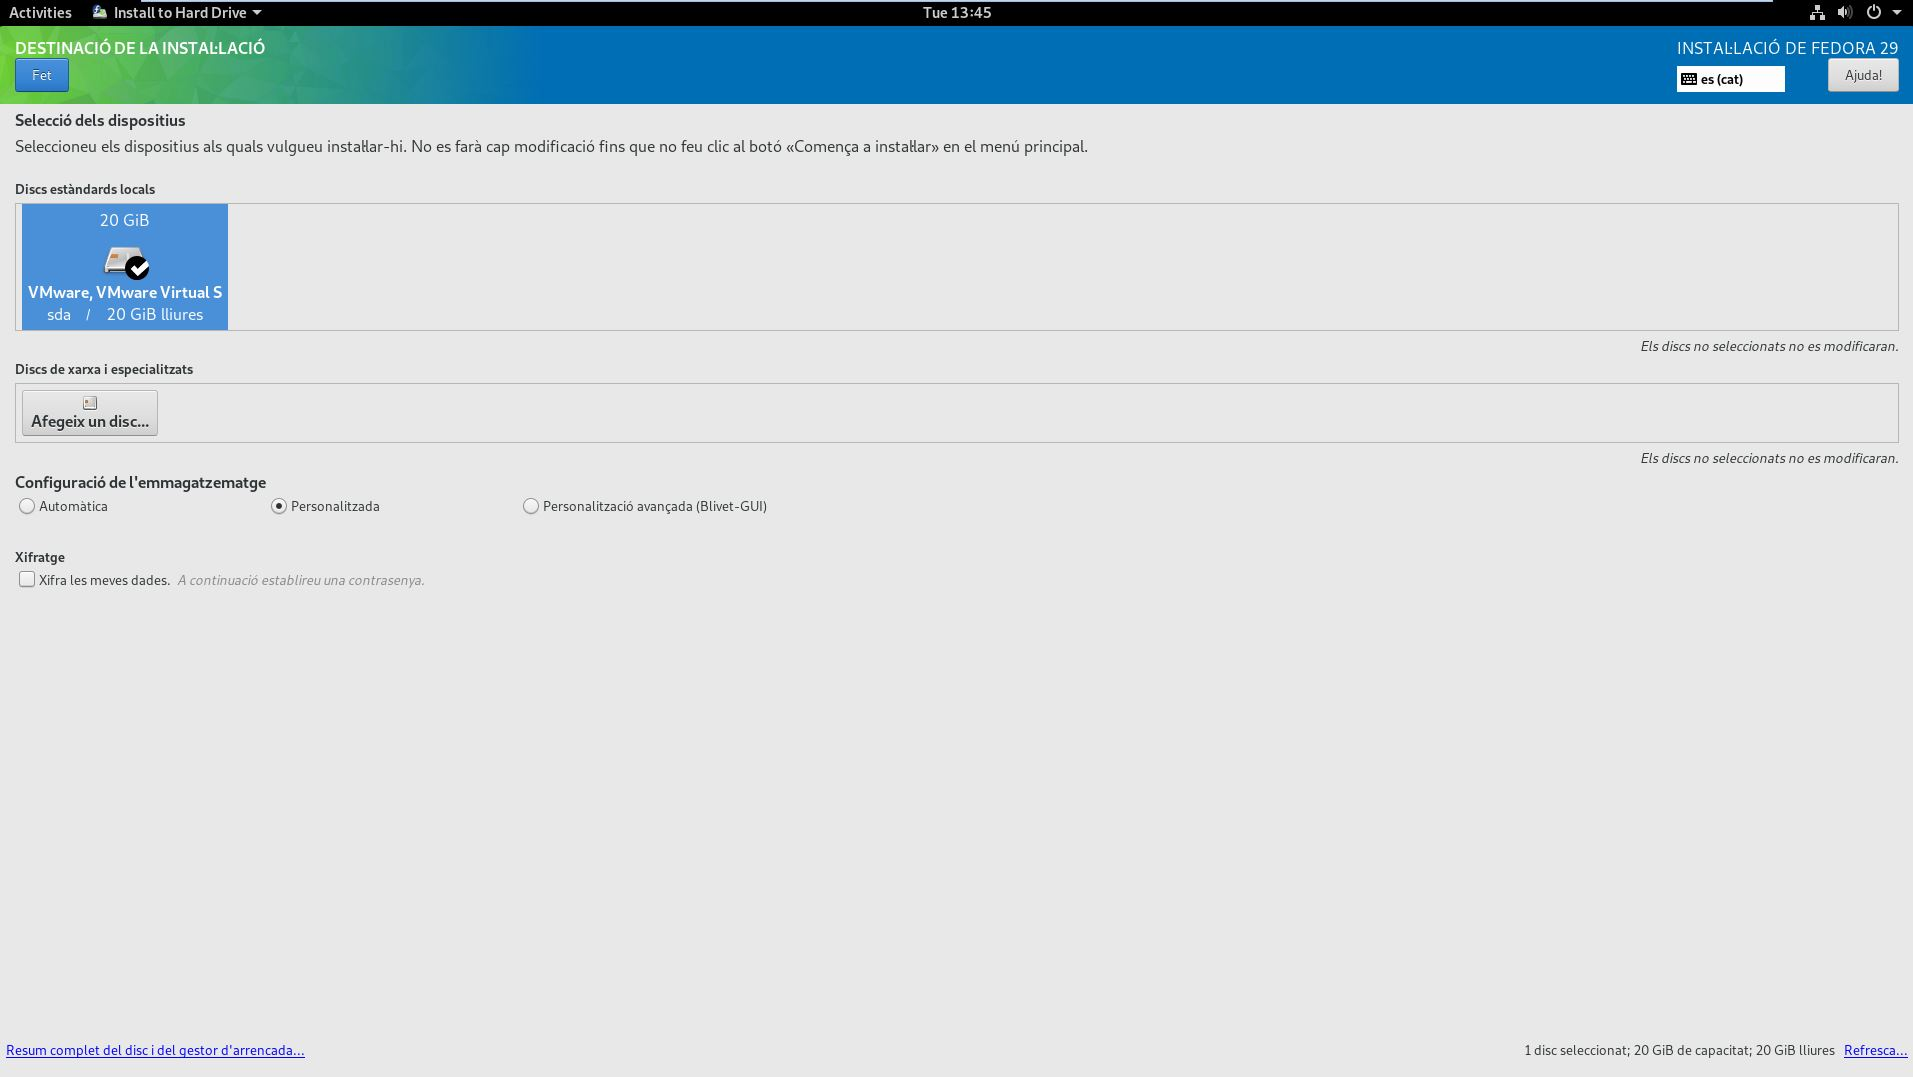
\includegraphics[width=11cm]{anex/fedora2.JPG}
    \end{center}
    \caption{Configuración del disco podemos dejarlo en automático personalizado vamos a realizar la misma configuración que con el ubuntu}
\end{figure}
\begin{figure}[!htbp]
    \begin{center}
        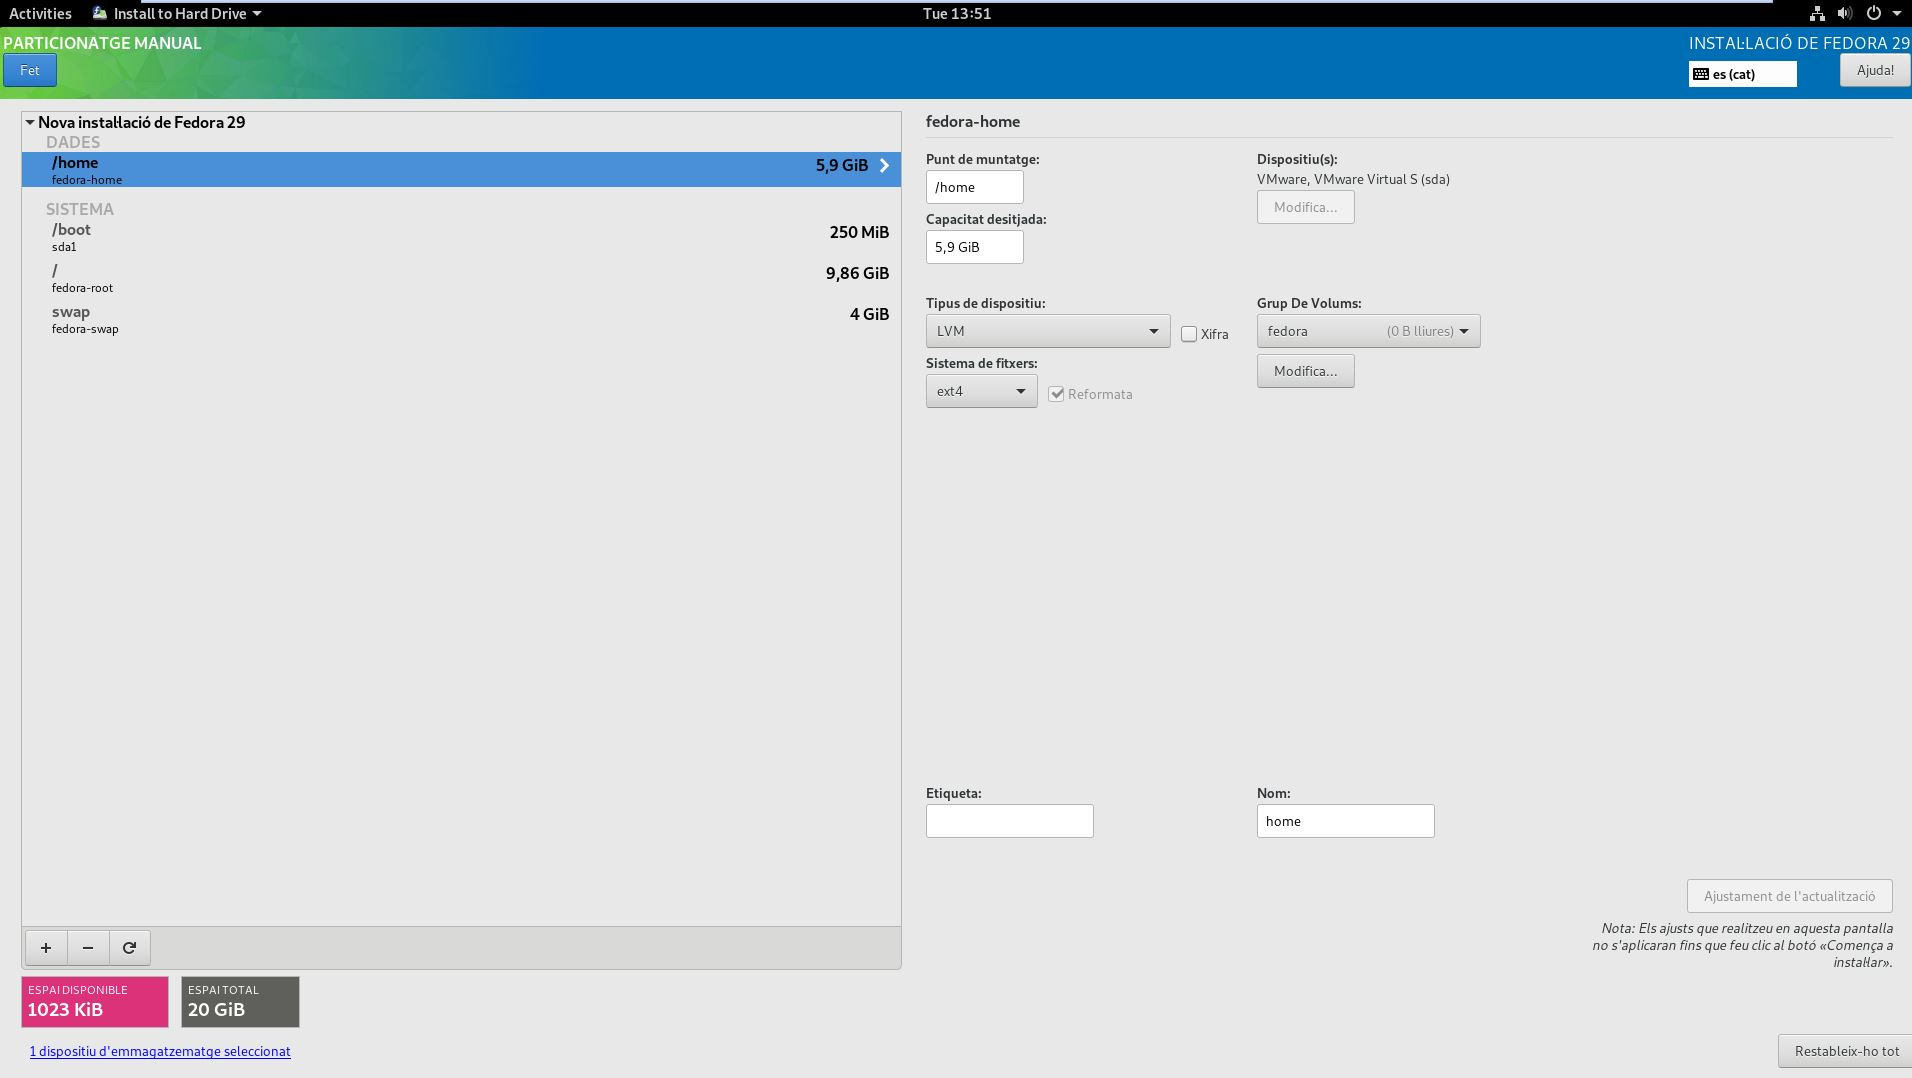
\includegraphics[width=11cm]{anex/fedora3.JPG}
    \end{center}
    \caption{Podemos configurar las particiones en el formato que queramos una partición para todo el sistema o frentes particiones para las carpetas generales}
    \begin{center}
        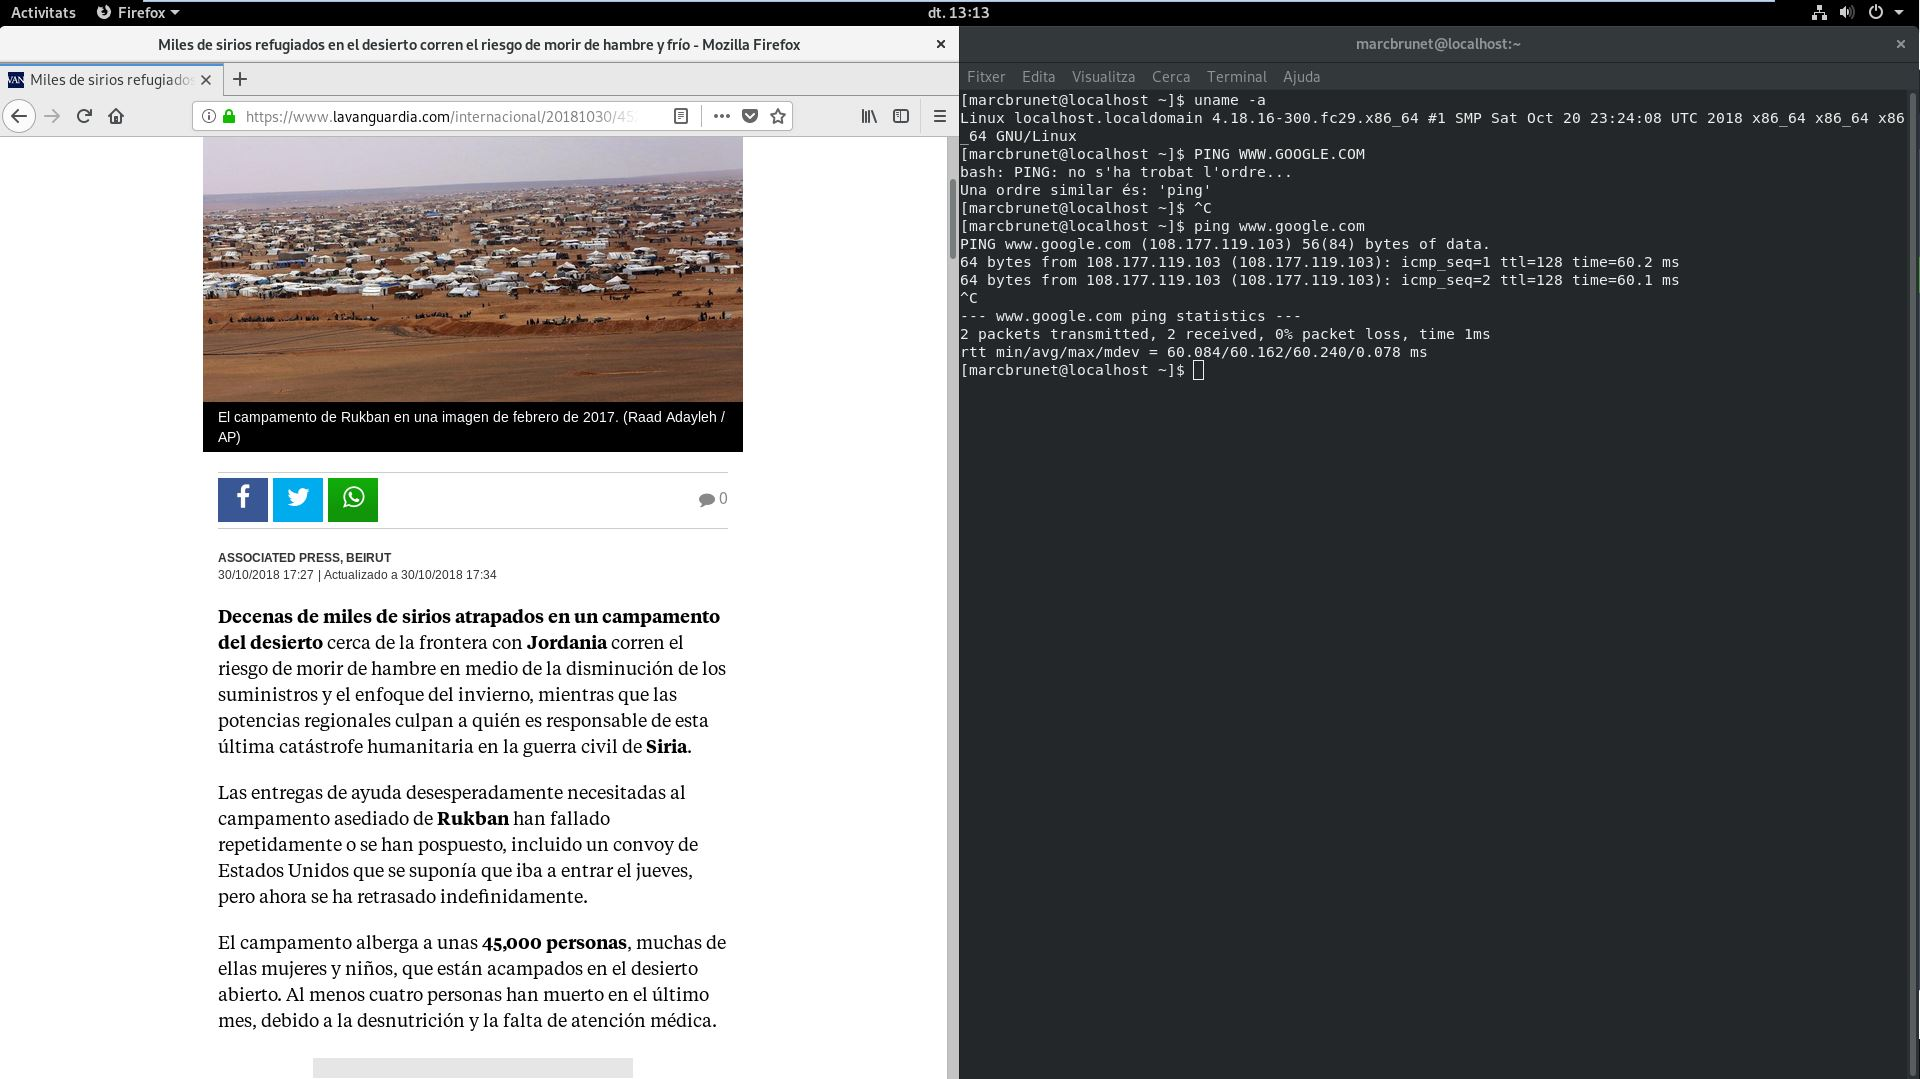
\includegraphics[width=11cm]{anex/fedora4.JPG}
    \end{center}
    \caption{Al iniciar nos pedirá la configuran del usuario y podremos comenzar a usar el sistema, ejecución del comando uname -a i ping + la vanguardia }
\end{figure}

\end{document}